\chapter{Approach}
\label{chapter3}
\thispagestyle{empty}

\section{Dynamic Binary Instrumentation}
\paragraph{}
Dynamic Binary Instrumentation is a technique for analysing the behaviour of a binary application through the injection of instrumentation code. The instrumentation code can be developed in an high level programming language and is executed in the context of the analysed binary with a granularity up to the single assembly instruction. The injection of instrumentation code is achieved by implementing a set of callbacks provided by the DBI framework. The most common and useful callbacks are:
\begin{itemize}
 \item Instruction callback: invoked for each instruction;
 \item Image load callback: invoked each time an image (dll or Main image) is loaded into memory;
  \item Thread start callback: invoked each time a thread is started;
\end{itemize}
Besides the callbacks the DBI framework allows to intercept and modify operative system APIs and system calls and this is very useful to track some behaviours of the binary, like the allocation of dynamic memory areas.


\section{Approach overview}
\paragraph{}
Our tool exploits the functionalities provided by the Intel PIN Dynamic Binary Instrumentation frameworks to track the memory addresses which are written and then executed with an instruction level granularity.
More in details for each instruction the following steps are performed:
\begin{enumerate}
\item Instruction Filtering: ignore the effects of a particular set of instructions for performance reasons;
\item Written addresses tracking: keep track of each memory address which is written in order to create a list of memory ranges of contiguous writes defined "Write Sets" .
\item Write xor execution instructions tracking: check if the currently executed instruction belongs to a "Write Set". This is a typical behaviour in a packer that is executing the unpacked layer and for this reason we trigger a detailed analysis which consists of:
	\begin{enumerate}
	\item Dumping the main image of the PE and a memory range on the heap depending on the address of the current instruction;
	\item Reconstructing the IAT and generating the correct  Import Directory;
	\item Applying some heuristics to evaluate if the current instruction is the Original Entry Point;
	\end{enumerate}
\end{enumerate}
The result of our tool is set of memory dumps or reconstructed PE depending on the result of the IAT fixing phase and a report which includes the values of each heuristics for every dump. Based on these information we can choose the best dump, that is the one that has the greatest chance of work.\\

\section{Approach details}
\paragraph{}
In this section we are going to describe in details the steps introduced in the previous section.
\paragraph{}
During the development we have adapted our approach in order to increase speed and effectiveness of our tool. Following there is a detailed explanation of our improvements on the initial approach:
\begin{enumerate}
\item in the first step, we add the option of not to track writes of library instructions on the stack and in the TEB
\item in the second step we filter instructions of known libraries before dumping
	\begin{enumerate}
	\item when trying to reconstruct the IAT we added some code in order to deal with 			obfuscation techniques like \textit{IAT Redirection} and \textit{Stolen API}
	\item our heuristics are:
		\begin{itemize}
		\item entropy: check if the value of the entropy is above a certain threshold
		\item long jump: check if the "distance" between the current EIP and the previous 			one is above a certain threshold
		\item jump outer section: check if the current EIP is a different section from the 		one of the previous EIP
		\item pushad popad: check is a pushad popad has been found in the trace
		\item init function calls: check if the imports of the dump are function commonly 			 used by the malware and not by the unpacking layers
		\end{itemize}
	\end{enumerate}
\end{enumerate} 
For the instructions that execute from the same write set we adopted the following approach: if the "distance" between the current EIP and the EIP of the previous instruction is above a given threshold then we do the same as if we were in the case 2, otherwise we jump to the next instruction.\\
Finally, we are noticed that dumping only the main executable in memory is not enough because some packers dump the final payload on the heap. In order to deal with it, we track heap allocations and writes inside an heap interval. If necessary, we dump these intervals too.

\subsection{Instruction Filtering}
\paragraph{}
Since our tool works with an instruction level granularity limiting our analysis to the relevant instruction of the program is a critical point. For this reason we have introduced some filters, based on the common behaviours showed by the packers, which make our tool ignore the effects of a set of instructions. More in detail two kind of instructions are not tracked by default:
\begin{itemize}
	\item Write instruction on the TEB and on the Stack;
	\item Instruction executed by known Windows Libraries;
\end{itemize}
The write instructions on the stack are ignored because unpacking code on the stack is not common compared to unpacking it on the heap or inside the main image. Moreover many instructions write on the stack and keeping track of all the written addresses would downgrade the performances gaining little advantages against a very small set of packers.\\
The same considerations can be applied to the instructions which write on the TEB, since most of these writes are related to the creation of instruction handlers and there is very little chance that a packer uses this addresses to unpack the encrypted payload.\\
The instructions executed by known Windows Libraries are never considered when checking if the current instruction address is contained inside a \textit{Write Set} because this would mean that the packer writes the malicious payload in the address space of a know Windows Library. This behaviour has never been identified in the packer analysed; moreover, this could introduce some crashes if the application explicitly use one of the functions which have been overwritten.

\subsection{Track WxorX instructions}
\paragraph{}
All packers, in order to work correctly, have to present a common behaviour: they must write the original program in memory and then they must execute the written code. We have defined an instruction that is first written by the packer and then executed as a \textit{WxorX instruction}.
Our tool tracks each write operation made by the program and build a set of memory ranges which identify contiguously written memory addresses. A memory range is dentified by a starting address and an end address and it is managed in order to take into account the memory operation that overlaps the it (The starting address and the end address are decreased or increased 
respectively when an overlapping writes is detected).

\begin{figure}[H]
 \makebox[\textwidth][c]{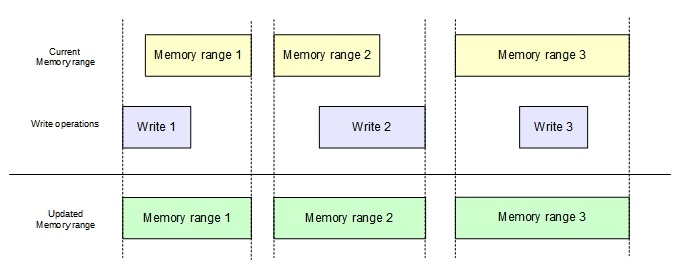
\includegraphics[width=1.0\textwidth]{./pictures/wxorx_tracking.jpg}}%
\caption{Memory range management}
\end{figure} 

The first time we detect that the instruction pointer is inside one of our memory ranges, all the analysis and dumping routines (explained in the next chapters) are triggered and the memory range is marked as \textit{broken}. It is easy to deduct that the definition of a broken memory range is : A memory range in which the execution has been redirected to. 